% We need layers to draw the block diagram
\pgfdeclarelayer{background}
\pgfdeclarelayer{foreground}
\pgfsetlayers{background,main,foreground}

% Define a few styles and constants
\tikzstyle{sensor}=[draw, fill=blue!20, text width=5em,text centered, minimum height=2.5em, rounded corners]
\tikzstyle{system} = [sensor, text width=5em, fill=green!30, 
    minimum height=8em]
%\tikzstyle{input} = [coordinate]
\tikzstyle{sum} = [draw, fill=blue!20, circle, node distance=1cm]
\tikzstyle{output} = [coordinate]
%\def\blockdist{0.5}
\def\edgedist{2.85}
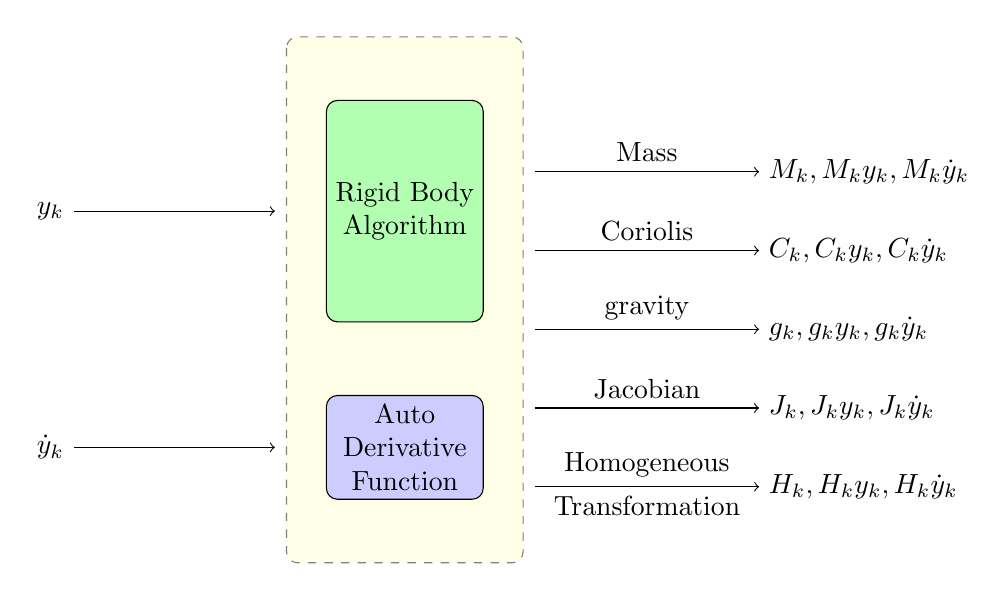
\begin{tikzpicture}
	% Define the nodes in the picture
	\node (y)[yshift=1cm]{$y_k$};
	\node (dy) [below of=y,node distance=3cm]{$\dot y_k$};
    \node (rigbdy_alg) [system,right of=y,node distance=4.5cm] {Rigid Body Algorithm};
    \node (auto_diff) [ sensor,below of=rigbdy_alg,node distance =3cm]{Auto Derivative Function};
    \node (M) [output,right of=rigbdy_alg,node distance=1.65cm,yshift=0.5cm]{};
    \node (C) [output,below of=M,node distance=1cm]{};
    \node (g) [output,below of=C,node distance=1cm]{};
    \node (J) [output,below of=g,node distance=1cm]{};
    \node (H) [output,below of=J,node distance=1cm]{};

    % Define the edges in the picture
    \draw [->] (y) --node{}+(\edgedist,0);
    \draw [->] (dy) --node{}+(\edgedist,0);
    \draw [->]  (M) --node[above]{Mass}+(\edgedist,0) node[right]{$M_k, \dfdx{M_k}{y_k},\dfdx{M_k}{\dot y_k}$};
    \draw [->]  (C) --node[above]{Coriolis}+(\edgedist,0) node[right]{$C_k, \dfdx{C_k}{y_k},\dfdx{C_k}{\dot y_k}$};
    \draw [->]  (g) --node[above]{gravity}+(\edgedist,0) node[right]{$g_k, \dfdx{g_k}{y_k},\dfdx{g_k}{\dot y_k}$};
    \draw [->]  (J) --node[above]{Jacobian}+(\edgedist,0) node[right]{$J_k, \dfdx{J_k}{y_k},\dfdx{J_k}{\dot y_k}$};
    \draw [->]  (H) --node[above]{Homogeneous} node[below]{Transformation}+(\edgedist,0) node[right]{$H_k, \dfdx{H_k}{y_k}, \dfdx{H_k}{\dot y_k}$};
    
    %Draw background layers
    \begin{pgfonlayer}{background}
        % Compute a few helper coordinates
        \path (auto_diff.west |- rigbdy_alg.north)+(-0.5,0.8) node (a) {};
        \path (auto_diff.south -| rigbdy_alg.east)+(+0.5,-0.8) node (b) {};
        \path[fill=yellow!10,rounded corners, draw=black!50, dashed]
            (a) rectangle (b);
    \end{pgfonlayer}
%\end{comment}
\end{tikzpicture}
